\chapter{Soluzione proposta}\label{soluzione-proposta}

La soluzione progettata consiste in un sistema di traduzione Text-to-SQL
ingegnerizzato per consentire l'interazione con diverse piattaforme di
database, prescindendo dalla conoscenza diretta del linguaggio SQL da
parte dell'utente. L'architettura si divide in due macro-componenti:
un'interfaccia utente (Frontend) sviluppata in React, concepita per
garantire un'interazione intuitiva e diretta, e un motore di
elaborazione (Backend) implementato in Python e strutturato in moduli
software esposti tramite endpoint grazie al framework FastAPI. Il codice
sorgente dell'intero sistema, comprensivo dei moduli di backend e
frontend, è stato reso disponibile pubblicamente su GitHub \cite{github_project}.

Il cuore logico del backend è governato da due orchestratori principali:
lo \texttt{SchemaOrchestrator} e il \texttt{QueryOrchestrator}. Tali
componenti hanno il compito di coordinare i vari moduli del sistema,
garantendo l'efficienza dei flussi d'esecuzione.

\section{Schema Orchestrator}\label{schema-orchestrator}

Lo \texttt{SchemaOrchestrator} è deputato principalmente
all'acquisizione, alla strutturazione e alla persistenza delle
informazioni relative allo schema del database relazionale di
destinazione. L'obiettivo centrale è generare un'istanza informativa
permanente che possa essere condivisa ed efficacemente consultata nel
corso delle diverse sessioni utente.

\subsection{Acquisizione dello schema}\label{acquisizione-dello-schema}

Il processo di acquisizione ha inizio verificando l'eventuale presenza
di una rappresentazione dello schema precedentemente salvata in formato
JSON. Qualora si renda necessaria una nuova estrazione, il sistema
prevede due scenari alternativi: l'estrazione diretta tramite un client
database (\texttt{database\_client}) o l'estrazione guidata tramite un
Modello Linguistico (LLM) sollecitato da un prompt ingegnerizzato.

Nel primo scenario, il sistema sfrutta il \texttt{database\_client}, una
classe specializzata nell'interazione nativa con il DBMS dell'utente,
capace di garantire la massima accuratezza informativa. Il client espone
il metodo \texttt{extract\_schema}, il quale interroga direttamente il
dizionario dei dati di sistema (es. la tabella
\texttt{information\_schema}) per recuperare i metadati relativi a
tabelle, colonne, tipi di dato e vincoli di integrità referenziale
(chiavi esterne). I dati della query di ispezione vengono
temporaneamente incapsulati in un oggetto \texttt{QuerySession} e
gestiti tramite un cursore di connessione. Al fine di garantire la
robustezza del software, il ciclo di vita della connessione prevede una
gestione delle eccezioni per intercettare fallimenti di runtime o
timeout d'esecuzione. Se l'operazione ha successo (\texttt{SUCCESS}), le
righe estratte vengono modellate in una struttura dati custom denominata
\texttt{Records}, per poi essere formattate e mappate nelle
corrispondenti posizioni del file JSON dello schema.

Nel \textbf{secondo scenario}, che si attiva qualora l'utente fornisca
file DDL o descrizioni testuali del database in linguaggio naturale,
l'interazione con i modelli generativi è governata da una gerarchia di
classi fondata sulla classe astratta \texttt{BaseLLM}. Quest'ultima
definisce l'interfaccia comune per tutti i connettori LLM del sistema,
esponendo il metodo astratto \texttt{generate(prompt,\ kwargs)} e
incapsulando proprietà condivise come il meccanismo di gestione del
timeout \texttt{TIMEOUT\_PER\_REQUEST}, impostato di default a dieci
minuti.

L'estensione di tale interfaccia è implementata tramite componenti
specializzate per i singoli provider:

\begin{itemize}
\item
  \textbf{AzureLLM:} si interfaccia nativamente con i servizi di Azure
  OpenAI sfruttando un loader interno (\texttt{AzureLoader}) per il
  recupero sicuro delle credenziali e degli endpoint. Il metodo
  \texttt{generate} esegue la chiamata verso le API di chat
  completion e incapsula l'operazione all'interno di un costrutto
  \texttt{try-except}, sollevando un'eccezione esplicita di
  \texttt{TimeoutError} qualora l'operazione superi la finestra
  temporale prefissata.
\item
  \textbf{OpenWebUILLM:} estende \texttt{BaseLLM} introducendo una
  flessibilità strutturale basata sull'attributo \texttt{api\_type}, che
  discrimina a runtime tra interfacce basate su chat (\texttt{chat}) e
  interfacce basate su completamento del testo (\texttt{completion}).
  Tale biforcazione logica viene gestita istanziando dinamicamente il
  loader configurativo appropriato (\texttt{ChatLoader} o
  \texttt{CompLoader}) per l'estrazione dei parametri di connessione e
  delle chiavi di autenticazione.
\end{itemize}

La gestione del ciclo di vita della richiesta in \texttt{OpenWebUILLM}
si appoggia sempre sul metodo \texttt{generate}, il quale inoltra una
richiesta HTTP POST sincrona verso l'endpoint configurato utilizzando la
libreria \texttt{requests}. Per far fronte alla natura duale dell'API,
la classe implementa due metodi privati dedicati:
\texttt{\_dynamic\_payload}, deputato alla generazione del corpo della
richiesta formattato con i parametri posizionali o con la cronologia dei
messaggi, e \texttt{\_dynamic\_response}, incaricato di eseguire il
parsing selettivo del dizionario JSON restituito dal server.

Un elemento di rilievo ingegneristico all'interno di
\texttt{\_dynamic\_response} è rappresentato dal meccanismo preventivo
di intercettazione degli errori di contesto. Mediante un'analisi
lessicale della risposta del server, il sistema verifica se l'anomalia
sia riconducibile al superamento dei limiti fisici della finestra di
contesto del modello, mappando token critici quali \texttt{n\_ctx} o
\texttt{context\ length}. In caso positivo, viene sollevata un'eccezione
mirata di \texttt{ValueError}, impedendo la propagazione di fallimenti
generici e fornendo un feedback strutturato ai moduli superiori
dell'applicazione. Infine, la conformità con la politica di tolleranza
ai guasti dell'architettura è preservata catturando esplicitamente le
eccezioni di tipo \texttt{requests.exceptions.Timeout}, che vengono
uniformate e rilanciate sotto forma di \texttt{TimeoutError}.

In questo caso, la classe \texttt{PromptBuilder} genera dinamicamente un
prompt (\texttt{schema\_generation\_prompt} \ref{acquisizione-dello-schema}) inserendo l'input
dell'utente in un contesto predefinito. Il prompt definisce il ruolo del
modello (esperto di basi di dati) e impone rigidi vincoli strutturali,
richiedendo espressamente un output in formato JSON valido, privo di
commenti o testo conversazionale generico.

Al fine di validare e rendere persistente il risultato ottenuto da
entrambi gli scenari, viene invocato il metodo privato
\texttt{\_process\_response}. Questo delega il parsing sintattico alla
componente \texttt{Schema} mediante il metodo \texttt{parse\_response}.
Per mitigare la variabilità e le imperfezioni tipiche degli output dei
modelli linguistici, il meccanismo di parsing effettua in sequenza
quattro strategie di recupero euristico:

\begin{itemize}
\item
  \textbf{Parsing JSON diretto:} tentativo di deserializzazione standard
  del testo.
\item
  \textbf{Isolamento tramite parentesi graffe:} estrazione del testo
  compreso tra la prima e l'ultima parentesi graffa, supportato da una
  pulizia automatica delle virgole terminali (trailing commas).
\item
  \textbf{Markdown Fenced Blocks:} estrazione del codice circoscritto
  dai tripli backtick (``\,').
\item
  \textbf{Widest Candidate:} ricerca iterativa del frammento JSON valido
  più esteso presente nel corpo del testo.
\end{itemize}

Una volta convalidata la struttura, il file JSON viene salvato
localmente. Contestualmente, lo \texttt{SchemaOrchestrator} invoca il
metodo \texttt{add\_schema} dello \texttt{SchemaStore} per indicizzare
le tabelle appena estratte all'interno del sistema RAG
(Retrieval-Augmented Generation). Il metodo
\texttt{to\_documents} converte i metadati di ciascuna tabella in
documenti compatibili con il vector store utilizzato. Durante questa
fase, eventuali documenti preesistenti riferiti allo stesso database
vengono preventivamente rimossi dallo store per evitare conflitti di
versione e garantire l'allineamento dei dati in caso di aggiornamento.

\subsection{Aggiornamento dello
schema}\label{aggiornamento-dello-schema}

Qualora l'utente desideri arricchire o modificare la conoscenza dello
schema, il sistema consente l'aggiornamento incrementale attraverso il
metodo \texttt{update\_current\_schema}. Previa verifica dell'esistenza
del file JSON di base, viene eseguita un'analisi euristica sull'input
dell'utente mediante il metodo \texttt{classify\_update}. Questo
analizza la presenza di specifiche parole chiave per determinare la
natura della modifica. Se l'aggiornamento non altera l'architettura dei
dati ma aggiunge dettagli descrittivi, il testo viene semplicemente
archiviato nel campo \texttt{semantic\_notes} della classe
\texttt{Schema}. Se l'input implica variazioni su tabelle o colonne,
viene strutturato un nuovo prompt di aggiornamento
(\texttt{schema\_update\_prompt} \ref{aggiornamento-dello-schema}) tramite il \texttt{PromptBuilder}.
Questo prompt include lo schema corrente e le istruzioni per integrare
le modifiche. La risposta dell'LLM viene infine processata nuovamente
dal metodo \texttt{\_process\_response}, garantendo la medesima catena
di validazione e persistenza utilizzata in fase di prima acquisizione.

\section{Query Orchestrator}\label{query-orchestrator}

Il \texttt{QueryOrchestrator} è il componente core deputato alla
traduzione semantica delle richieste formulate dall'utente in linguaggio
naturale in istruzioni SQL eseguibili. Ereditando i metadati strutturali
precedentemente consolidati dallo \texttt{SchemaOrchestrator}, questo
modulo implementa un ciclo iterativo di generazione, valutazione e
raffinamento che consente al sistema di correggere i propri output
analizzando i fallimenti d'esecuzione.

All'atto dell'inizializzazione, l'orchestratore riceve come
parametri l'identificativo del database, un'istanza dello
\texttt{SchemaStore}, il modello linguistico selezionato e,
opzionalmente, il modulo \code{database_client}. La presenza o
l'assenza di quest'ultimo determina una biforcazione logica nel
flusso elaborativo, discriminando la possibilità di effettuare o
meno una validazione dinamica e sperimentale sul DBMS dell'utente.
In fase di istanziazione, l'orchestratore si avvale del design
pattern Factory tramite la classe \texttt{LLMFactory}, il cui
metodo statico \texttt{create} esamina il dizionario di
configurazione per isolare le specifiche del provider (come chiavi
crittografiche ed endpoint di connessione) e restituire il
corrispondente wrapper specializzato (\texttt{BaseLLM}).

\subsection{Generazione e Raffinamento Iterativo della
Query}\label{generazione-e-raffinamento-iterativo-della-query}

Il processo principale è governato dal metodo \texttt{generation}, il
cui obiettivo consiste nell'esaminare la richiesta e restituire un
oggetto \texttt{QuerySession} contenente il codice SQL finale e i
metadati associati al ciclo di vita della sessione. Tramite il metodo
privato \texttt{\_init\_generation\_context}, il sistema interroga lo
\texttt{SchemaStore} per ricavare la porzione di schema rilevante
(\texttt{schema\_context}). Al fine di ottimizzare la finestra di
contesto dell'LLM ed evitare l'inclusione di tabelle superflue, lo store
applica un'euristica basata sulla stima della complessità dell'input.
Analizzando la presenza di specifici costrutti linguistici riconducibili
a operazioni di aggregazione o di join, il sistema espande dinamicamente
il parametro di recupero \(k\) partendo da un valore basale (\(k=3\))
fino a un massimo di 7 tabelle. I documenti così selezionati dal vector
store vengono de-duplicati e formattati. Qualora sia disponibile una
connessione attiva tramite il \code{database_client}, il contesto
viene ulteriormente integrato mediante due sorgenti informative
fondamentali:

\begin{itemize}
\item
  Analisi dei Fallimenti Pregressi (\texttt{QueryStore})\emph{:} Il
  sistema interroga un secondo database vettoriale (\texttt{QueryStore})
  contenente lo storico delle query fallite. Tramite una ricerca per
  similarità semantica combinata con una funzione di decadimento
  temporale (che predilige gli errori più recenti), vengono estratti
  fino a 3 documenti associati a tentativi precedentemente
  contrassegnati da uno stato di errore (es. \texttt{SYNTAX\_ERROR} o
  \texttt{RUNTIME\_ERROR}). Tali elementi vengono passati come vincolo
  negativo all'LLM per impedirgli di ripetere il medesimo errore logico.
\item
  Suggerimenti di Join (\texttt{join\_hints})\emph{:} Sfruttando le
  capacità introspettive del \code{database_client}, l'orchestratore
  interroga i metadati di sistema (quali
  \texttt{information\_schema.KEY\_COLUMN\_USAGE}) per mappare le
  relazioni di chiave esterna attive tra le tabelle coinvolte nella
  richiesta. L'output, tradotto in una lista di vincoli strutturali,
  guida esplicitamente il modello nella stesura delle clausole di
  \texttt{JOIN}.
\end{itemize}

Completata la fase di recupero del contesto, il sistema avvia un ciclo
iterativo di ottimizzazione governato da soglie rigide volte a prevenire
loop infiniti o un consumo eccessivo di token. Il ciclo si interrompe
non appena la query viene validata con successo o, in alternativa, al
raggiungimento di 5 errori di runtime consecutivi
(\texttt{runtime\_error\_limit}) o di 3 riscontri semantici negativi
(\texttt{evaluation\_attempts\_limit}).

La formulazione del codice SQL per ogni singolo tentativo è
demandata al metodo \code{_generate_sql_attempt}, il quale
invoca la classe \texttt{PromptBuilder} generando il prompt
ingegnerizzato \code{query_generation_prompt} \ref{lst:prompt_query_gen}. Il testo generato
organizza rigorosamente la richiesta dell'utente, il dialetto SQL
di destinazione, lo schema estratto, i suggerimenti sulle chiavi
esterne, lo storico dei fallimenti e, infine, un piano logico
strutturato che impone al modello di determinare internamente le
tabelle necessarie e le relazioni d'aggiornamento prima di emettere
esclusivamente il codice SQL finale.

Alla ricezione della stringa testuale prodotta dal server dell'LLM,
viene avviata una routine di sanificazione sintattica
(\texttt{clean\_sql\_from\_llm}) all'interno dell'oggetto
\texttt{QuerySession}. Questa operazione è necessaria per eliminare i
frequenti artefatti dei modelli linguistici, rimuovendo blocchi di
codice Markdown, espressioni\ di\ controllo\ spurie\ (es.`\textless0x0A\textgreater`)
e troncando qualsiasi testo esplicativo successivo all'ultimo punto e
virgola.

La fase critica di verifica prevede due scenari determinati
dall'architettura d'istanziazione:

\begin{itemize}
\item
  \textbf{Assenza di Client Database:} La valutazione si limita alla
  verifica formale e sintattica della stringa mediante un parser
  astratto (\texttt{sqlglot}), il quale accerta l'assenza di violazioni
  grammaticali nella struttura SQL.
\item
  \textbf{Presenza di Client Database:} Viene invocato il metodo
  \texttt{evaluation}, che esegue direttamente la query sul database
  bersaglio impostando un timeout di sicurezza sul cursore d'esecuzione.
  In caso di successo, il risultato viene sottoposto a una seconda
  valutazione semantica demandata a un modello valutatore, deputato a
  verificare se le righe ottenute rispondano fedelmente alla domanda
  iniziale. In caso di fallimento ripetuto a runtime, il valutatore
  genera un feedback esplicativo sulle cause del problema che verrà
  iniettato nell'iterazione successiva.
\end{itemize}

Al termine di ciascun tentativo, il metodo \texttt{evaluate} classifica
formalmente la sessione valorizzando lo stato finale
(\texttt{QueryStatus}), la categoria dell'anomalia (\texttt{ErrorType})
e il dominio di competenza dell'errore (\texttt{KnowledgeScope}),
isolando i problemi puramente sintattici da quelli strutturali (es.
clausole \texttt{GROUP\ BY} mancanti) o strettamente legati ai vincoli
dello schema.

Infine, ogni transazione viene registrata all'interno del
\texttt{QueryStore} corredata da un set esteso di metadati (timestamp,
numero di tentativi, categorie d'errore ed esito del DBMS). Tale
storicizzazione assicura l'apprendimento continuo del sistema,
permettendo all'orchestratore di capitalizzare l'esperienza accumulata e
di restituire, alla chiusura del ciclo, la sessione d'ispezione più
efficiente ed accurata.

\begin{figure}
  \centering
  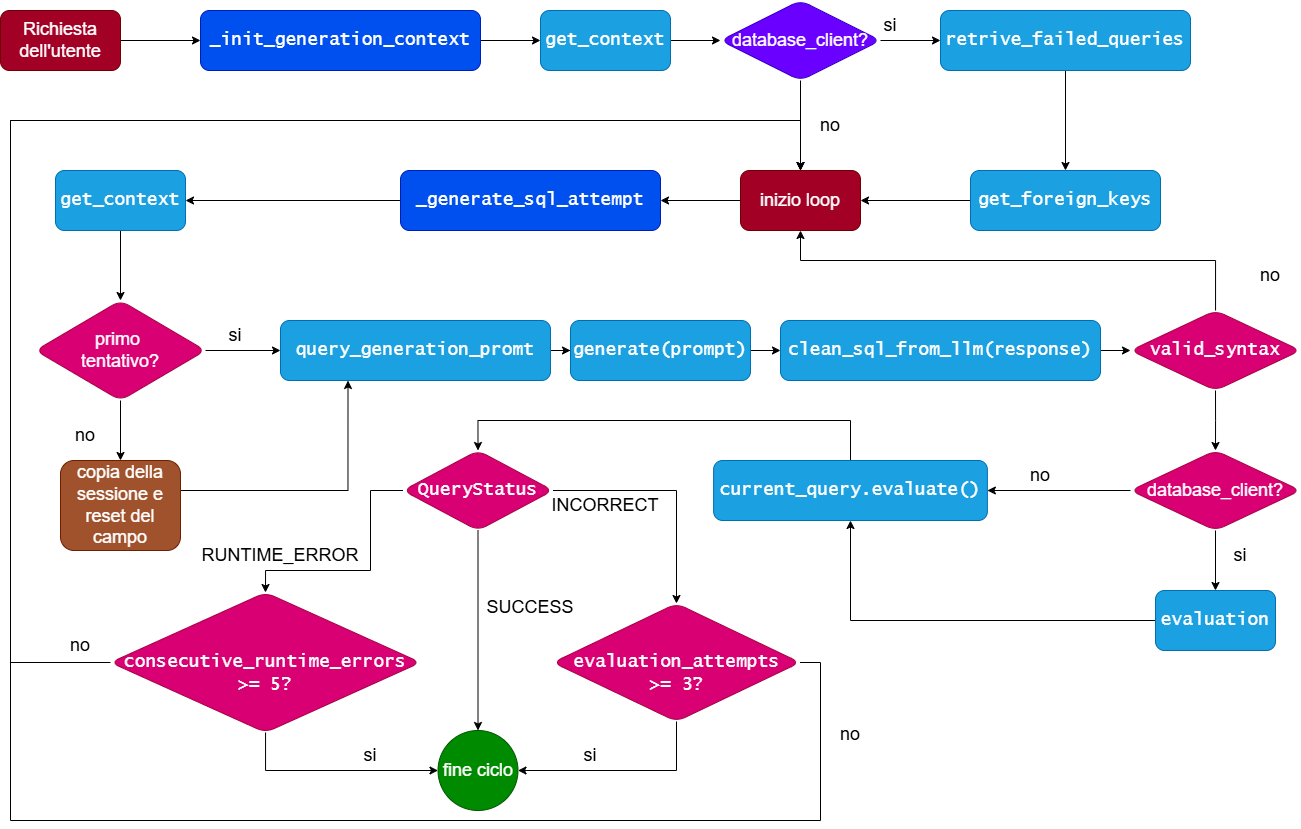
\includegraphics[width=0.80\textwidth]{immagini/workflows/generation.png}
  \caption{Flusso iterativo della generazione del codice SQL.}
\end{figure}

\subsection{Valutazione della query}\label{valutazione-della-query}

Il metodo \texttt{evaluation} presiede alla verifica formale, esecutiva
e semantica della query SQL generata. Questo processo di validazione
approfondita è subordinato alla disponibilità del
\code{database_client}, elemento indispensabile per interagire
direttamente con l'ambiente DBMS di destinazione e raccogliere i
riscontri empirici d'esecuzione.

All'avvio del modulo, la query candidata viene eseguita sul database
dell'utente. L'esito di tale operazione determina l'attivazione di due
circuiti di feedback distinti, gestiti in sinergia con un modello
linguistico indipendente configurato con il ruolo di valutatore
(LLM Evaluator).

Qualora l'esecuzione sul database fallisca a causa di un'eccezione del
DBMS, il sistema differisce l'intervento dell'LLM valutatore e
incrementa immediatamente il contatore interno degli errori di runtime
(\texttt{runtime\_errors}). Se l'anomalia persiste nelle iterazioni
successive, viene attivata una contromisura deterministica: la classe
\texttt{PromptBuilder} formula un prompt di spiegazione
(\texttt{explanation\_prompt} \ref{lst:prompt_explanation}) che isola la richiesta iniziale, il
codice SQL errato e il tracciato dell'eccezione restituito dal database.
L'LLM Evaluator analizza questo contesto per generare una diagnosi
mirata del fallimento. Tale risposta viene strutturata come un vincolo
correttivo e iniettata dinamicamente nel prompt di generazione del
tentativo successivo, guidando il modello di generazione verso la
risoluzione del bug sintattico o strutturale.

In caso di esecuzione riuscita della query, il sistema deve accertare
che i dati estratti rispondano fedelmente all'intento originario
dell'utente, scongiurando il rischio di query sintatticamente valide ma
logicamente errate. A tal fine, viene strutturato un prompt di
valutazione (\texttt{evaluation\_prompt} \ref{lst:prompt_evaluation}) che include la richiesta in
linguaggio naturale, il codice SQL prodotto e un campione
rappresentativo dei dati estratti, limitato ai primi venti record
(\texttt{Records.get\_preview}) per ottimizzare l'occupazione della
finestra di contesto del modello. L'LLM Evaluator esamina la coerenza
tra la struttura dei dati ottenuti e la semantica della domanda. Qualora
il verdetto sia positivo, lo stato della sessione (\texttt{QueryStatus})
viene consolidato come \texttt{SUCCESS}, interrompendo l'algoritmo
iterativo e restituendo la query validata.

Al termine di ciascuna iterazione, le metriche di classificazione e i
verdetti emessi dall'Evaluator vengono storicizzati all'interno
dell'oggetto \texttt{QuerySession}, alimentando la base di conoscenza
del \texttt{QueryStore} per i successivi cicli di recupero del contesto.

\section{Interfaccia}\label{interfaccia}

A completamento dell'architettura di backend descritta, è stata
sviluppata un'interfaccia utente dedicata, progettata per astrarre la
complessità dei processi di orchestrazione e fornire un punto di accesso
semplificato alle funzionalità di generazione e valutazione SQL.
L'applicazione frontend è strutturata in diverse viste logiche,
accessibili tramite una barra di navigazione persistente che include le
sezioni Home, Database e Generate.

La sezione dedicata alla gestione dei database rappresenta il
punto di innesco per lo \code{SchemaOrchestrator}. L'obiettivo di
questa interfaccia è permettere all'utente di definire il contesto
relazionale su cui opereranno i modelli di linguaggio. Il sistema
offre due modalità operative distinte. L'utente può caricare file di
definizione dati (DDL) o inserire manualmente istruzioni
\texttt{CREATE\ TABLE}. In questa modalità, l'interfaccia delega al
sistema l'inferenza della struttura tramite LLM per la produzione
dello schema JSON. Invece sfruttando il \texttt{MySQLClient},
l'utente può stabilire una connessione attiva con un server MySQL.
L'interfaccia presenta dinamicamente una lista dei database
accessibili, permettendo la selezione puntuale del target.

In entrambi i casi, l'utente è tenuto a specificare degli identificativi
mnemonici (il nome logico all'interno dell'applicazione e l'alias da
utilizzare nelle query) per garantire la corretta risoluzione dei
riferimenti durante la generazione del prompt. Una volta confermati i
dati, lo schema viene normalizzato, indicizzato nel \texttt{SchemaStore}
(Vector Database) e iniettato nella sessione attiva.

%%%%%%%%%%%%%%%%%%%%%%%%%%%%%%%%%% schema_mysql & schema_text %%%%%%%%%%%%%%%%%%%%%%%%%%%%%%%%%%

La pagina di generazione costituisce l'interfaccia di controllo del
\texttt{QueryOrchestrator}. Attraverso questa vista, l'utente può
configurare i parametri della sessione di interrogazione:

\begin{enumerate}
\def\labelenumi{\arabic{enumi}.}
\item
  \textbf{Selezione del Contesto:} Scelta del database tra quelli
  precedentemente configurati nella sessione.
\item
  \textbf{Configurazione del Modello:} Selezione del Large Language
  Model (LLM) tramite la \code{LLMFactory}, permettendo di
  testare la generazione su provider differenti (es. Azure o
  OpenWebUI).
\item
  \textbf{Input in Linguaggio Naturale:} Un'area di testo dedicata
  accoglie la richiesta dell'utente.
\end{enumerate}

%%%%%%%%%%%%%%%%%%%%%%%%%%%%%%%%%% generation %%%%%%%%%%%%%%%%%%%%%%%%%%%%%%%%%%

Al termine del processo di generazione, l'interfaccia non si limita a
mostrare il codice SQL prodotto, ma fornisce un feedback immediato
sull'efficacia della query. Se il database è stato collegato tramite
connessione diretta, il sistema esegue automaticamente la query e
presenta un'anteprima dei record estratti. Questo approccio
permette all'utente di validare istantaneamente non solo la correttezza
sintattica, ma anche la pertinenza semantica dei risultati rispetto alla
domanda originale.

Dalla Dashboard principale (Home), l'utente può indirizzare il workflow
verso due direttrici funzionali:

\begin{itemize}
\item
  \textbf{Generate Query:} Focalizzata sulla creazione ex-novo di
  codice SQL a partire da requisiti testuali.
\item
  \textbf{Evaluate Query:} Dedicata alla revisione critica di query
  esistenti, dove il sistema agisce come supervisore esperto per
  identificare errori logici o strutturali, sfruttando la logica di
  cross-check tra richiesta originale e metadati dello schema.
\end{itemize}

L'anteprima dell'interfaccia è presente nell'allegato